%=========================================================================
% (c) 2011, 2012 Josef Lusticky

\chapter{Design and analysis}
For implementation of reasonably useful NTP client,
operating system must be able to set, get
and eventually adjust the system time in a similar fashion as
described in section~\ref{sec:system-keeping-and-providing} and~\ref{sec:system-discipline}.
Though not mandatory, adjusting time is important function,
if the time shall be always a monotonically increasing function.
Apart from that, communicating abilities over UDP are also required.

For developing and testing Contiki NTP client,
the AVR Raven platform with 8-bit ATmega1284P CPU~\cite{avr-datasheet} will be used.
This platform features IEEE~802.15.4 (Low-Rate Wireless Personal Area Networks) link layer support.
Together with an adaptation layer called 6LoWPAN (IPv6 over Low power Wireless Personal Area Networks)
AVR Raven is able to communicate over IPv6.

How to get a working setup with Contiki on this platform is described in
the document files on the CD enclosed to this thesis.
The CD content hierarchy is listed in appendix~\ref{app:cd-content}.

%Older x86 processors used an interrupt mechanism to switch from
%user-space to kernel-space, but new x86 processors provide instructions
%that optimise this transition (using sysenter and sysexit instructions)~\cite{ibm-linux-system-calls}.
%... This is not in Contiki, as operating systems targeted at embbeded systems produce only 1 binary file. CITATION

%=========================================================================
% (c) 2011, 2012 Josef Lusticky

\section{Network communication}
Thanks to uIP, described in section~\ref{sec:contiki-uip},
the network communication is not a matter for Contiki OS.

intended to be used between different processes

AVR Raven features IEEE~802.15.4 (Low-Rate Wireless Personal Area Networks) link layer support.
On top of this layer, an adaptation layer called 6LoWPAN (IPv6 over Low power Wireless Personal Area Networks)
is used to communicate over IPv6 by Contiki.

Figure~\ref{fig:design-6lowpan} shows a complete hierarchy of network layers
concerned with NTP communication.
\begin{figure}
  \centering
  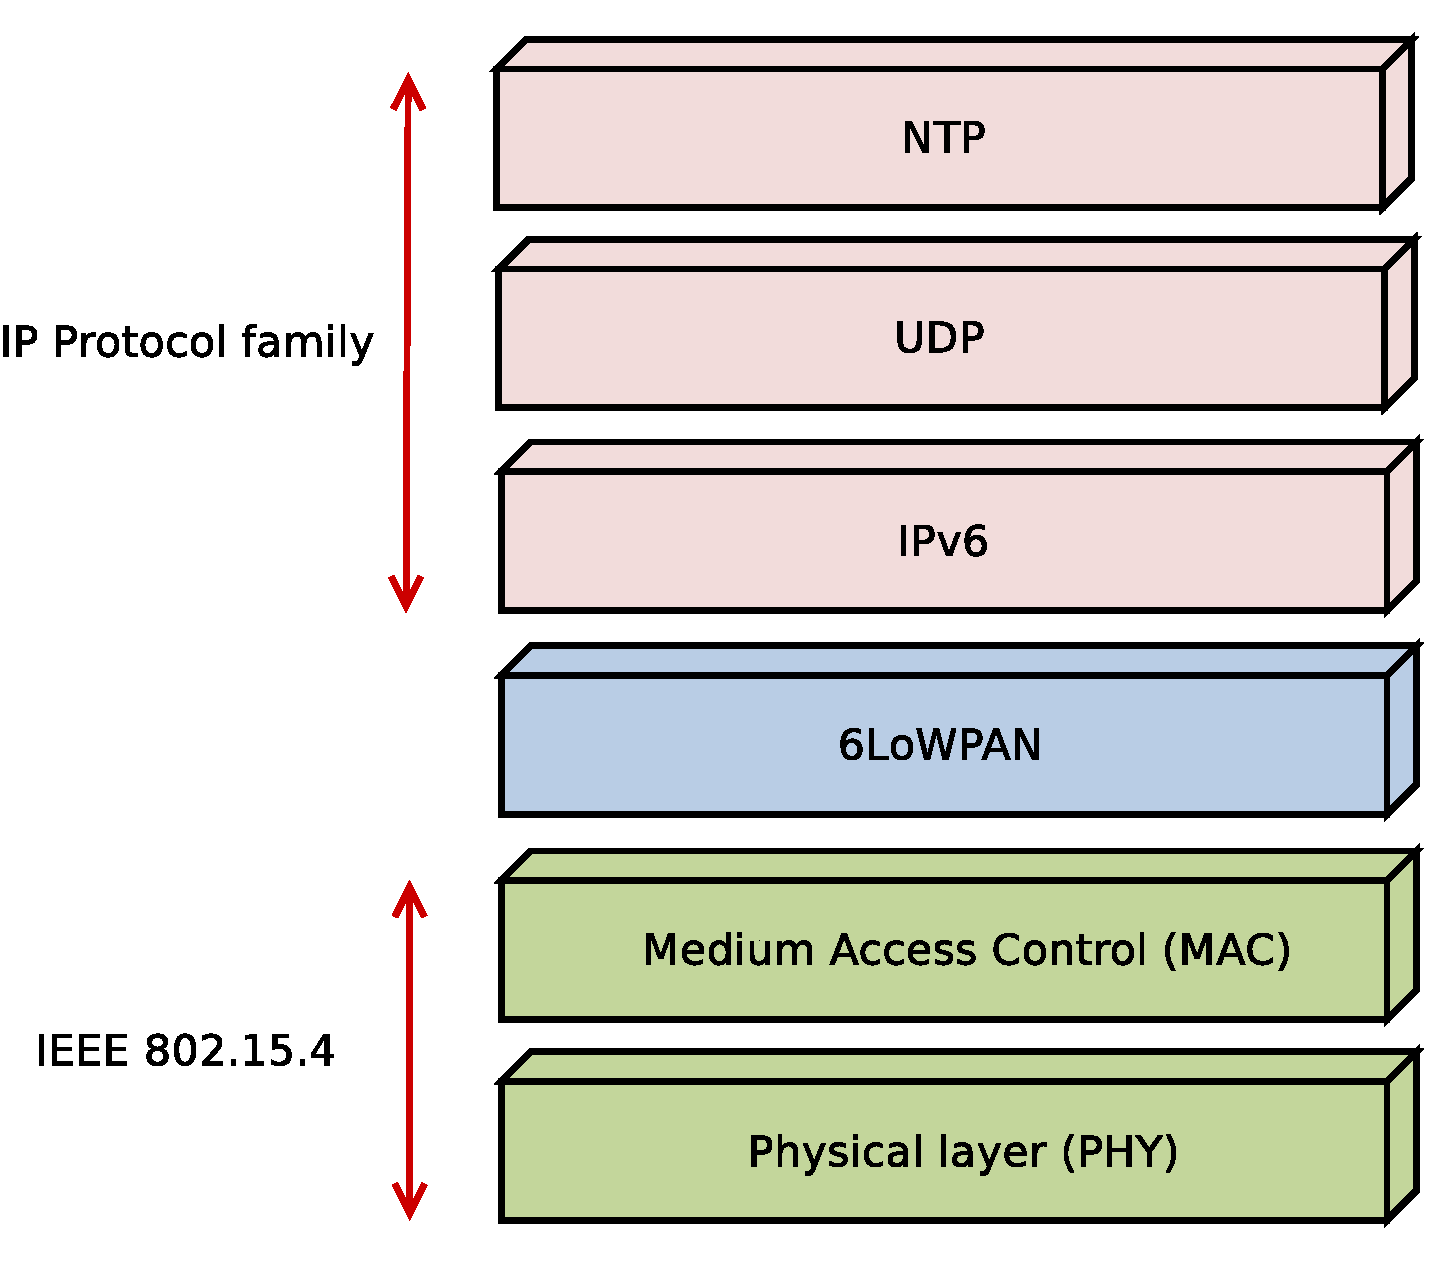
\includegraphics[width=9cm,keepaspectratio]{fig/6lowpan.pdf}
  \caption{Communication stack with 6lowpan layer}
  \label{fig:design-6lowpan}
  \bigskip
\end{figure}




%%=========================================================================
% (c) 2011, 2012 Josef Lusticky

\section{Time interface extension}\label{sec:analysis-interface}
Section~\ref{sec:analysis-time} described, that there is no proper
way of setting, getting and adjusting the time for an NTP client in Contiki OS.
A new interface for setting, getting and eventually adjusting the time
must be therefore developed.

Setting the time should not cause a misbehaviour of the Contiki timers
described in section~\ref{sec:analysis-time}.
A modification of the {\it{scount}} and the {\it{seconds}} variable must be therefore avoided.
This can be achieved using an additional variable, containing the system boot time,
and modifying only that variable by the call for setting the time.
This way, the {\it{seconds}} variable will be further representing the system uptime
and the current real time can be obtained by $boottime + seconds$.
Since the {\it{scount}} also can not be changed, setting the time is only possible
within a precision of one second.
%Finer time setting must be made using the time adjustments.

By contrast, a call for getting the current time must be able to provide a higher precision.
Therefore, a new time specification structure must be designed as well.
To conform to the POSIX standard~\cite{posix}, this structure should consist of two parts -
one representing seconds and the other representing nanoseconds.
The first part represents the number of elapsed seconds since the POSIX epoch.
The nanosecond precision was chosen as modern systems also aim towards this
precision~\cite{posix,ntp-precision} and
the microsecond precision would also require at least 32-bit data type -
one second has 1~000~000 microseconds, which is more than the maximum expressible value of
an unsigned 16-bit data type $2^{16}$-1 (65~535).

The call for getting the time fills the time specification structure.
The part representing seconds is simply filled with the value of $boottime + seconds$,
while the part representing nanoseconds should be filled with the maximum precision
the clock model allows.
As described in section~\ref{sec:analysis-time},
this can be achieved by reading the {\it{scount}} variable
and by querying the hardware counter that is used for
interrupt generation and includes the time passed since
the last update of the {\it{scount}} variable.
This way, the resolution of
$\frac{1}{CLOCK\_SECOND~\times~counts} = \frac{1}{128~\times~32} = 0.000244140625$~seconds
can be acquired,
where $counts$ is the number of counter register increments between two successive interrupts,
which is 32 by default on AVR Raven, as stated in section~\ref{sec:analysis-clock-interface}.
%If this part was filled by only using the {\it{scount}} variable,
%just the resolution of the timer interrupt frequency would be provided.

Since setting the current time is possible only within one second precision,
finer time setting must be made using the time adjustments.
Section~\ref{sec:analysis-time} explained, that adjusting the time
should use the hardware clock as much as possible.
Adjusting the time changes the value in {\it{OCR2A}} compare register
to delay or shorten the clock tick interval,
which in turn speeds up or slows down the system time.
If the amount of required adjustments is positive, then the system clock is speeded up
until the adjustment has been completed.
If the amount of required adjustments is negative, then the clock is slowed down in a similar fashion.
Since the application specifies the amount of adjustments by the timestamp,
a new call must be developed for the determination of how many
clock ticks will be delayed or shortened, respectively.

As a result of this design, a leap second occurrence will be handled like an unexpected change of time -
the operating system will continue with the wrong system time for some time,
but an NTP client will set or adjust the system time~\cite{ntp-faq}.
This will effectively cause the leap second correction to be applied too late,
what is a trade-off for smaller memory requirements.


